\subsection{Tools Used}
The model was designed using MATLAB\textregisteredmark\ and SIMULINK\textregisteredmark\ R2018B. Analysis was also performed using this software. Additionally, to aid testing, a generic video file was used provided by \hyperlink{https://blogs.unity3d.com/2016/11/28/free-vfx-image-sequences-flipbooks/}{Unity3D}.
\subsection{Assumptions}
The video file used has dimensions of 400x400px. Inside the parameters of certain blocks in the SIMULINK\textregisteredmark\ file this assumption was used and the model will need to be altered to work with video files of other dimensions. Additionally, the input video file was 30fps which is assumed in the frame counter module.
\subsection{Design}
The top level design is shown in Fig. \ref{fig:sysSpecs}. A general overview of this design is presented in this section with in-depth descriptions in later sections.
\begin{figure}[H]
    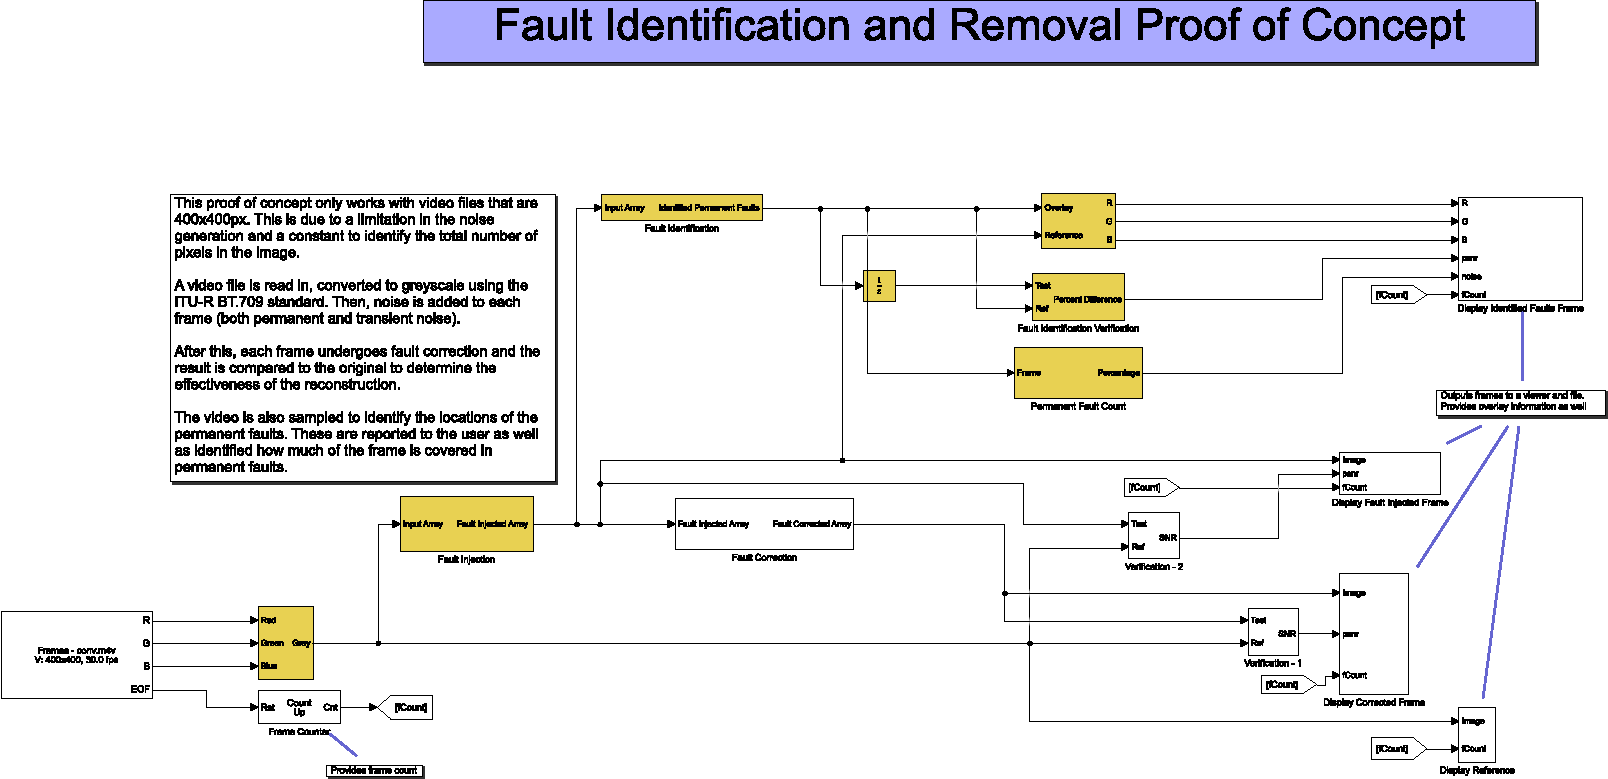
\includegraphics[width=\linewidth]{impl_dsgn}
    \caption{Top Level System Design}
    \label{fig:sysSpecs}
\end{figure}
\par An input video is fed into the \verb!From Multimedia File! block. Each color frame is converted to black and white to make image processing easier. Additionally, the \verb!EOF! output of the \verb!From Multimedia File! is fed into a frame counter's reset port, which is reset every time the video is restarted.
\par From this point, the video is sent to a noise generation unit. Since this model is a proof of concept, it is important to have a reference video as well as a video file with noise added. The noise generation block adds both permanent and transient noise.
\par After the frame has noise added, it is sent to two blocks, one to identify permanent noise in the frame, and another to filter out the noise in the frame.
\par Post noise generation, noise filtering, noise identification, and the reference frames are output to a video display as well as logged to a video file throughout simulation. Frame count information as well as other diagnostic and verification information is overlaid on top of the video frames to aid in analysis.
\subsubsection{ITU-R BT.709 Sub module}
The black and white conversion module follows the ITU-R BT.709 standard for color to black and white conversion. A reproduction of this module along with the coefficients used for each channel is shown in Fig. \ref{fig:btu709}.
\begin{figure}[H]
    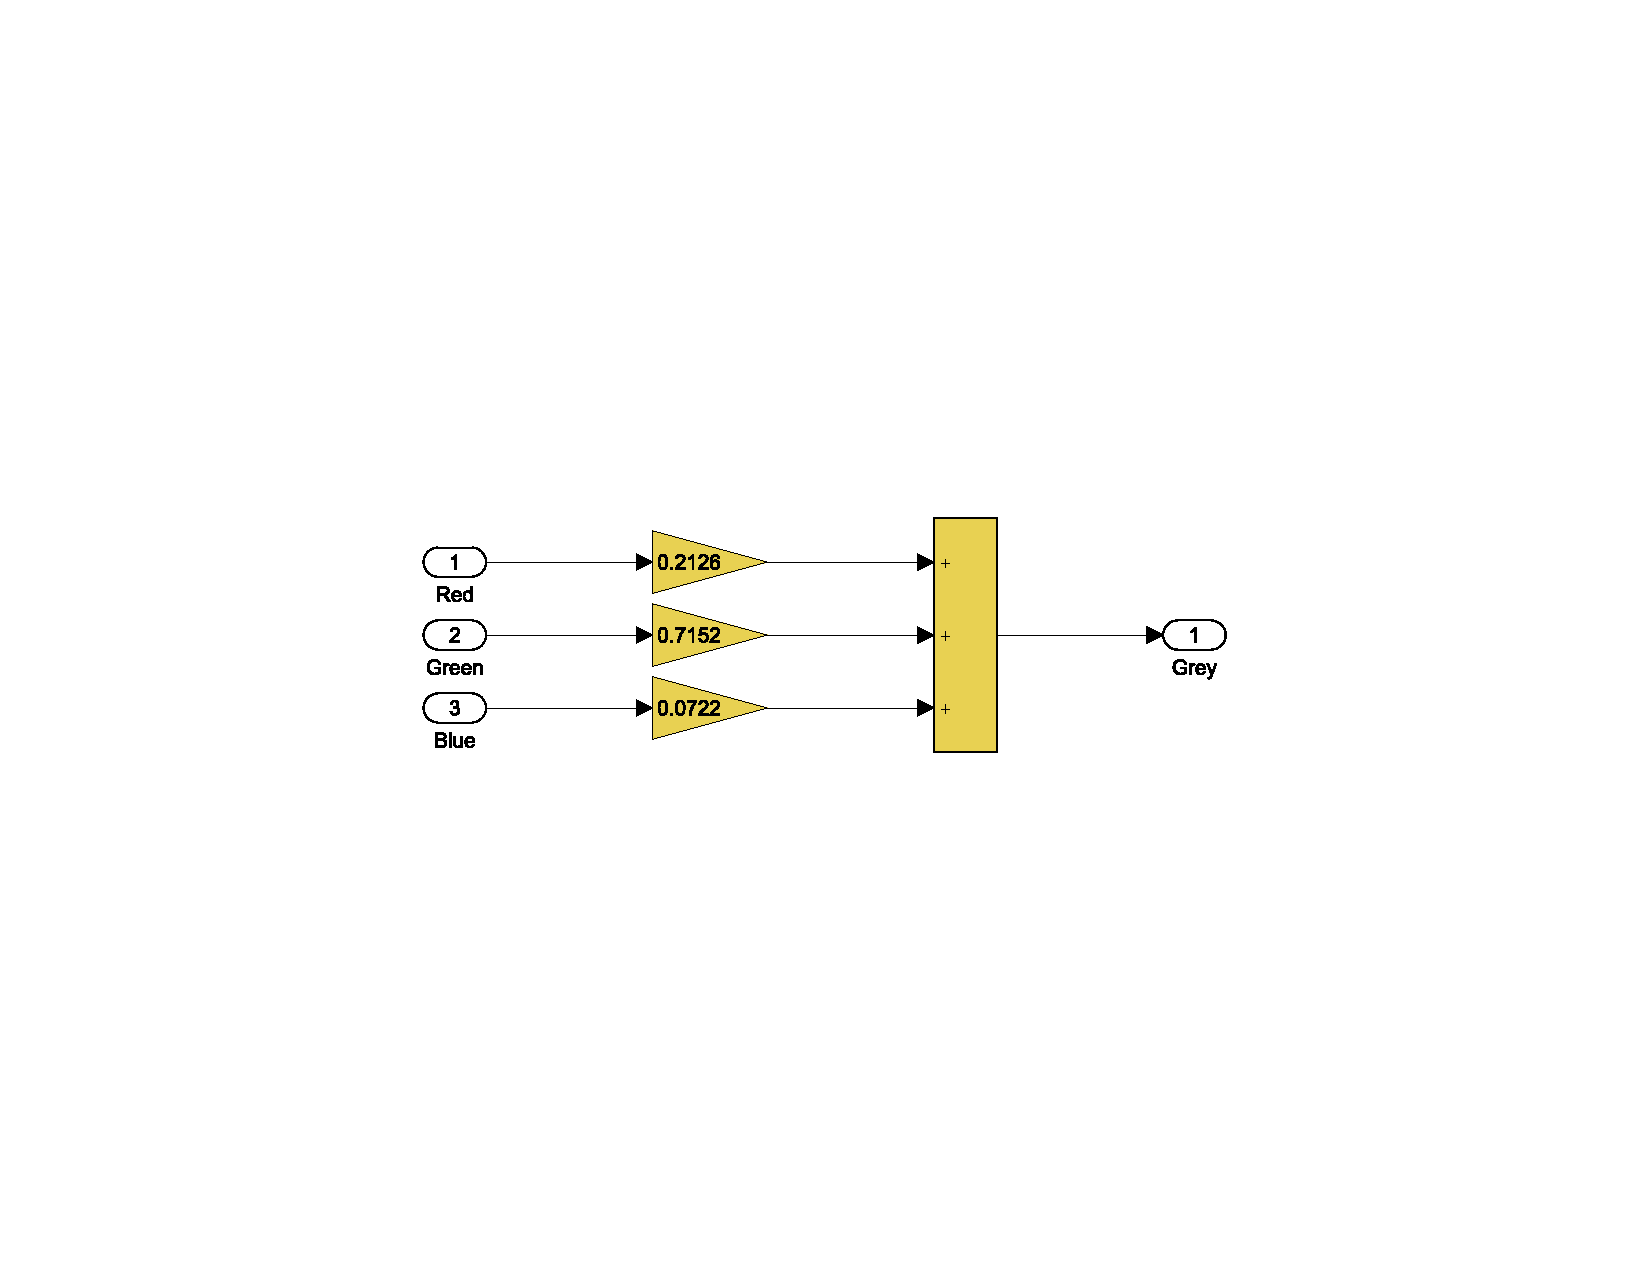
\includegraphics[width=\linewidth]{impl_dsgn_ITU-R BT.709}
    \caption{ITU-R BT.709 Color to Black and White Conversion}
    \label{fig:btu709}
\end{figure}

\subsubsection{Noise Generator Sub module}
The Noise generator generates both permanent and transient noise.
\begin{figure}[ht!]
    \subfloat[Top Level Noise Generator Block\label{fig:1a:topLevelNoiseGenerator}]{%
       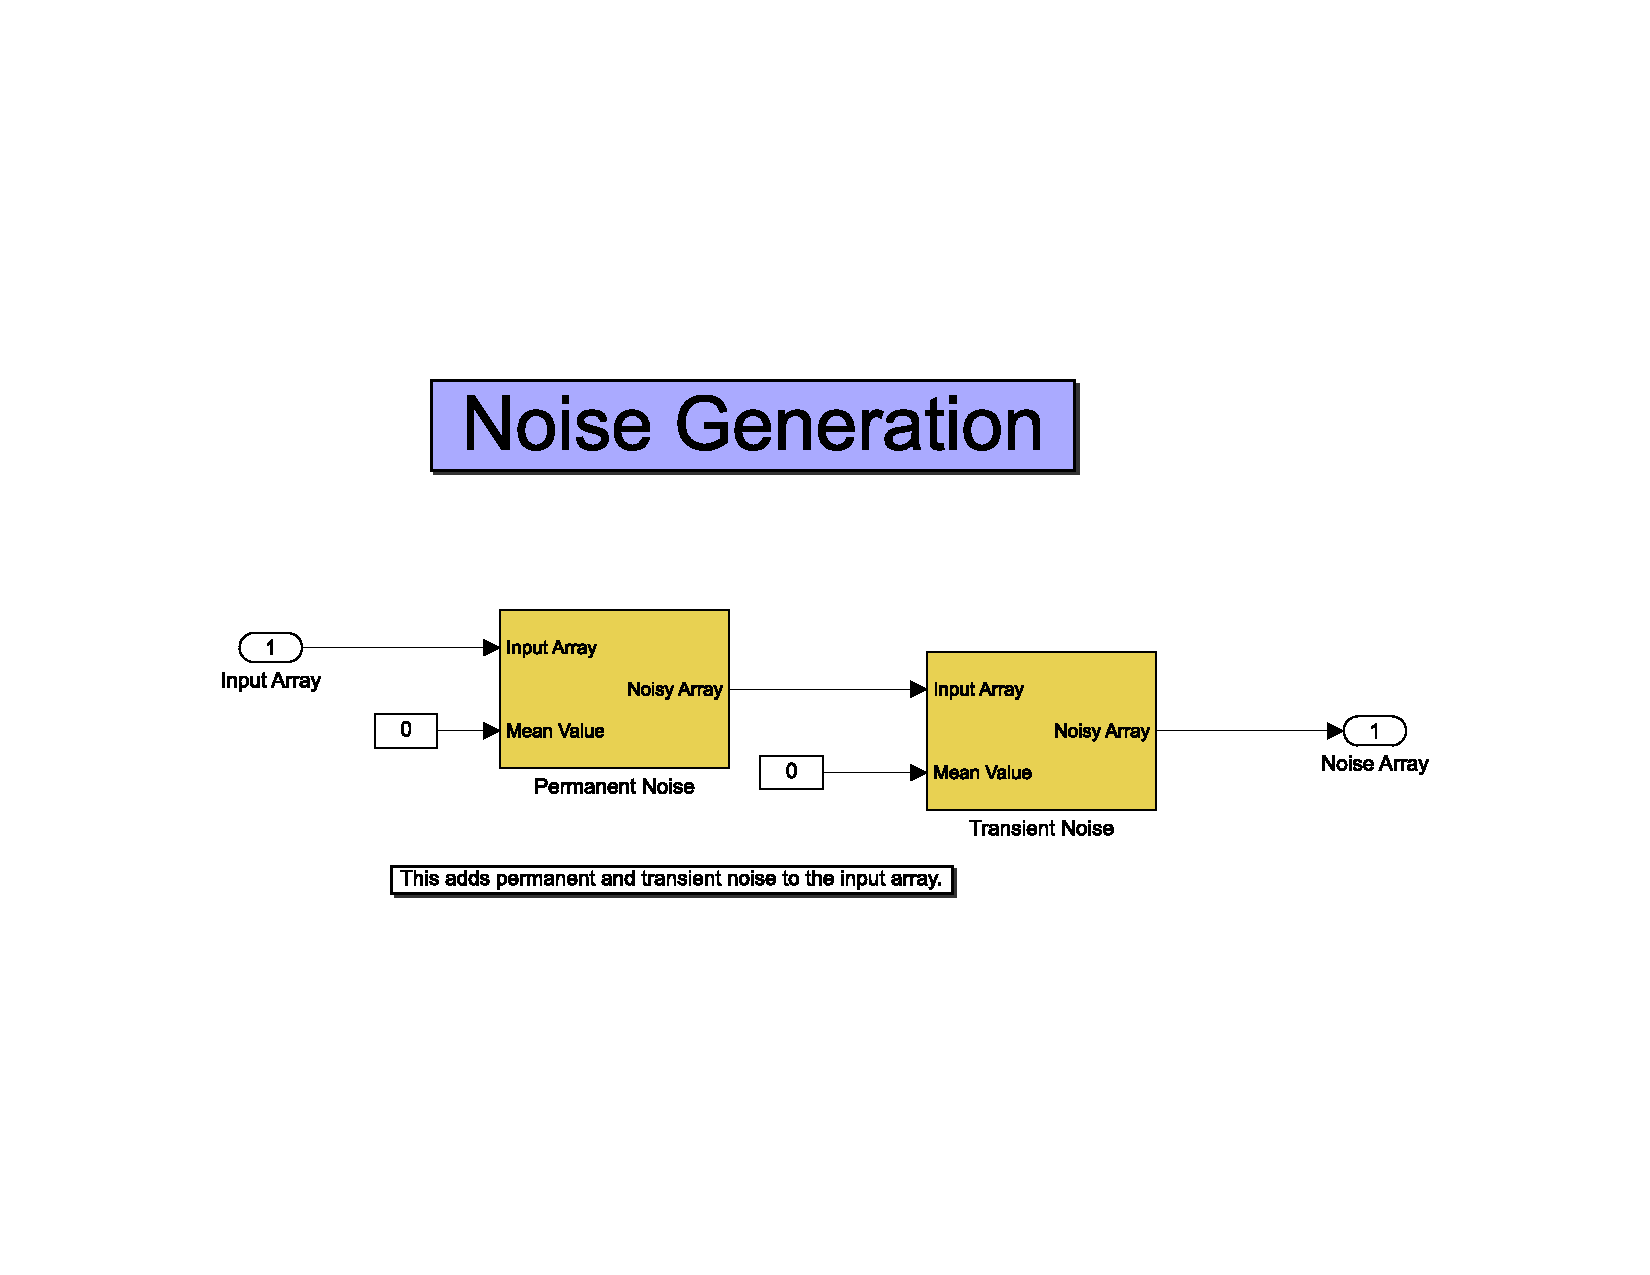
\includegraphics[width=\linewidth]{impl_dsgn_Noise Generator}}
    \\
     \subfloat[Permanent Noise Generator Block\label{fig:1b:permanentNoiseGenerator}]{%
        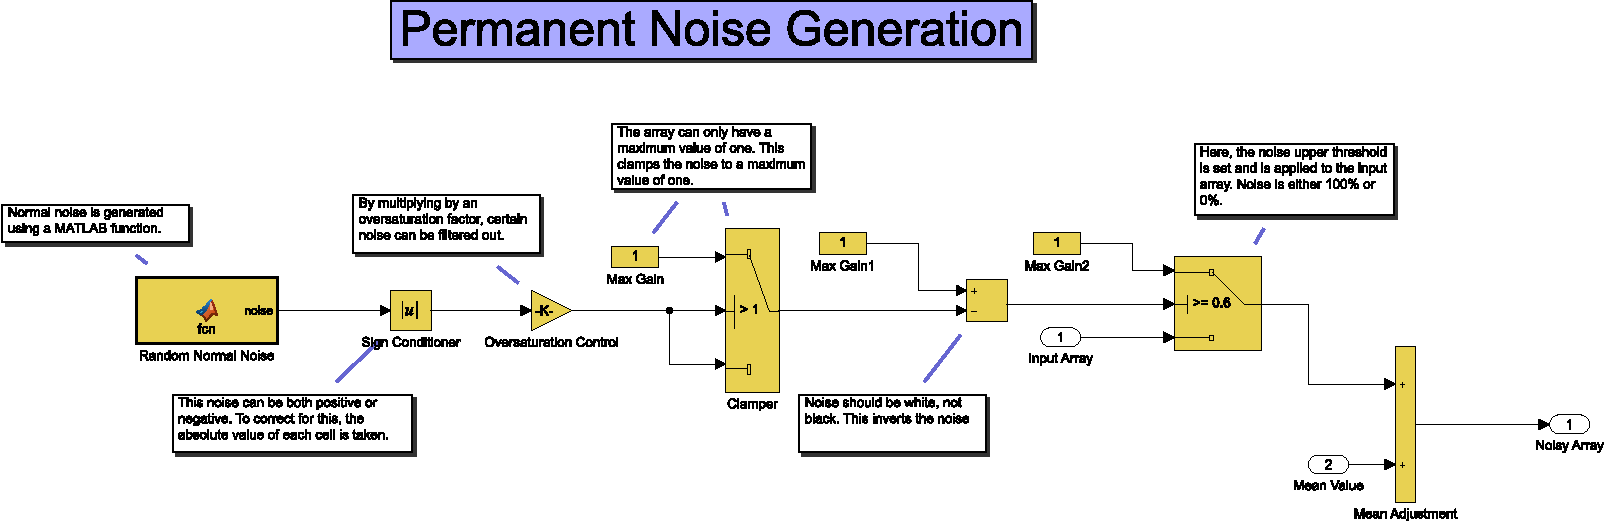
\includegraphics[width=\linewidth]{impl_dsgn_Noise Generator_Permanent Noise}}
    \caption{(a), (b) Shown are the top level noise generator block and the permanent noise generation block. The transient noise generation block is visually identical to the permanent noise generation block. The difference is inside of the MATLAB\textregisteredmark\ function block, and therefore was omitted.}
    \label{fig:noiseGenerator}
\end{figure}
\par As shown in Fig. \ref{fig:1a:topLevelNoiseGenerator}, the reference video frame is fed into the permanent noise generation block and then is fed into the transient noise generation block. Both the transient noise and permanent noise overlays are calculated each frame which results in an decrease in real-time performance of the demo. The transient noise generation block accounted for approximately 67\% of the total execution time followed next by the permanent noise generation block at approximately 3.2\% of the total execution time.
\par Noise is generated using the MATLAB\textregisteredmark\ \verb!randn! function. For the permanent noise, the seed is set to a fixed value of 100, and for the transient noise, the seed is set to \verb!shuffle! which sets the seed based off the current time to provide different noise each frame. This function is hard-coded to output a 400x400 matrix due to limitations in SIMULINK\textregisteredmark. The output of this matrix are values from the standard distribution, which can output both positive and negative values. Since pixel faults (and noise) can only be positive, the output matrix is corrected using an absolute value block. Next, since the maximum grey-scale value is one, a clamping block clamps the noise values to a maximum of one. The over-saturation control allows for more or less noise in the output matrix.
\par Until this point, the noise is black. The value one is subtracted from each cell in the matrix to invert the color (and make each value white). After this, the simulated image faults are added to the input array. Since a pixel can only be "on" or "off", a switch is used to selectively turn pixels on or off depending on the noise value threshold. Lastly, a mean value adjustment can be applied to the output matrix. For this application, the mean was set to zero so as not to alter the original image catastrophically.

\subsubsection{Noise Filtering Sub module}
Noise filtering is accomplished by using a modified median filter.
\begin{figure}[H]
    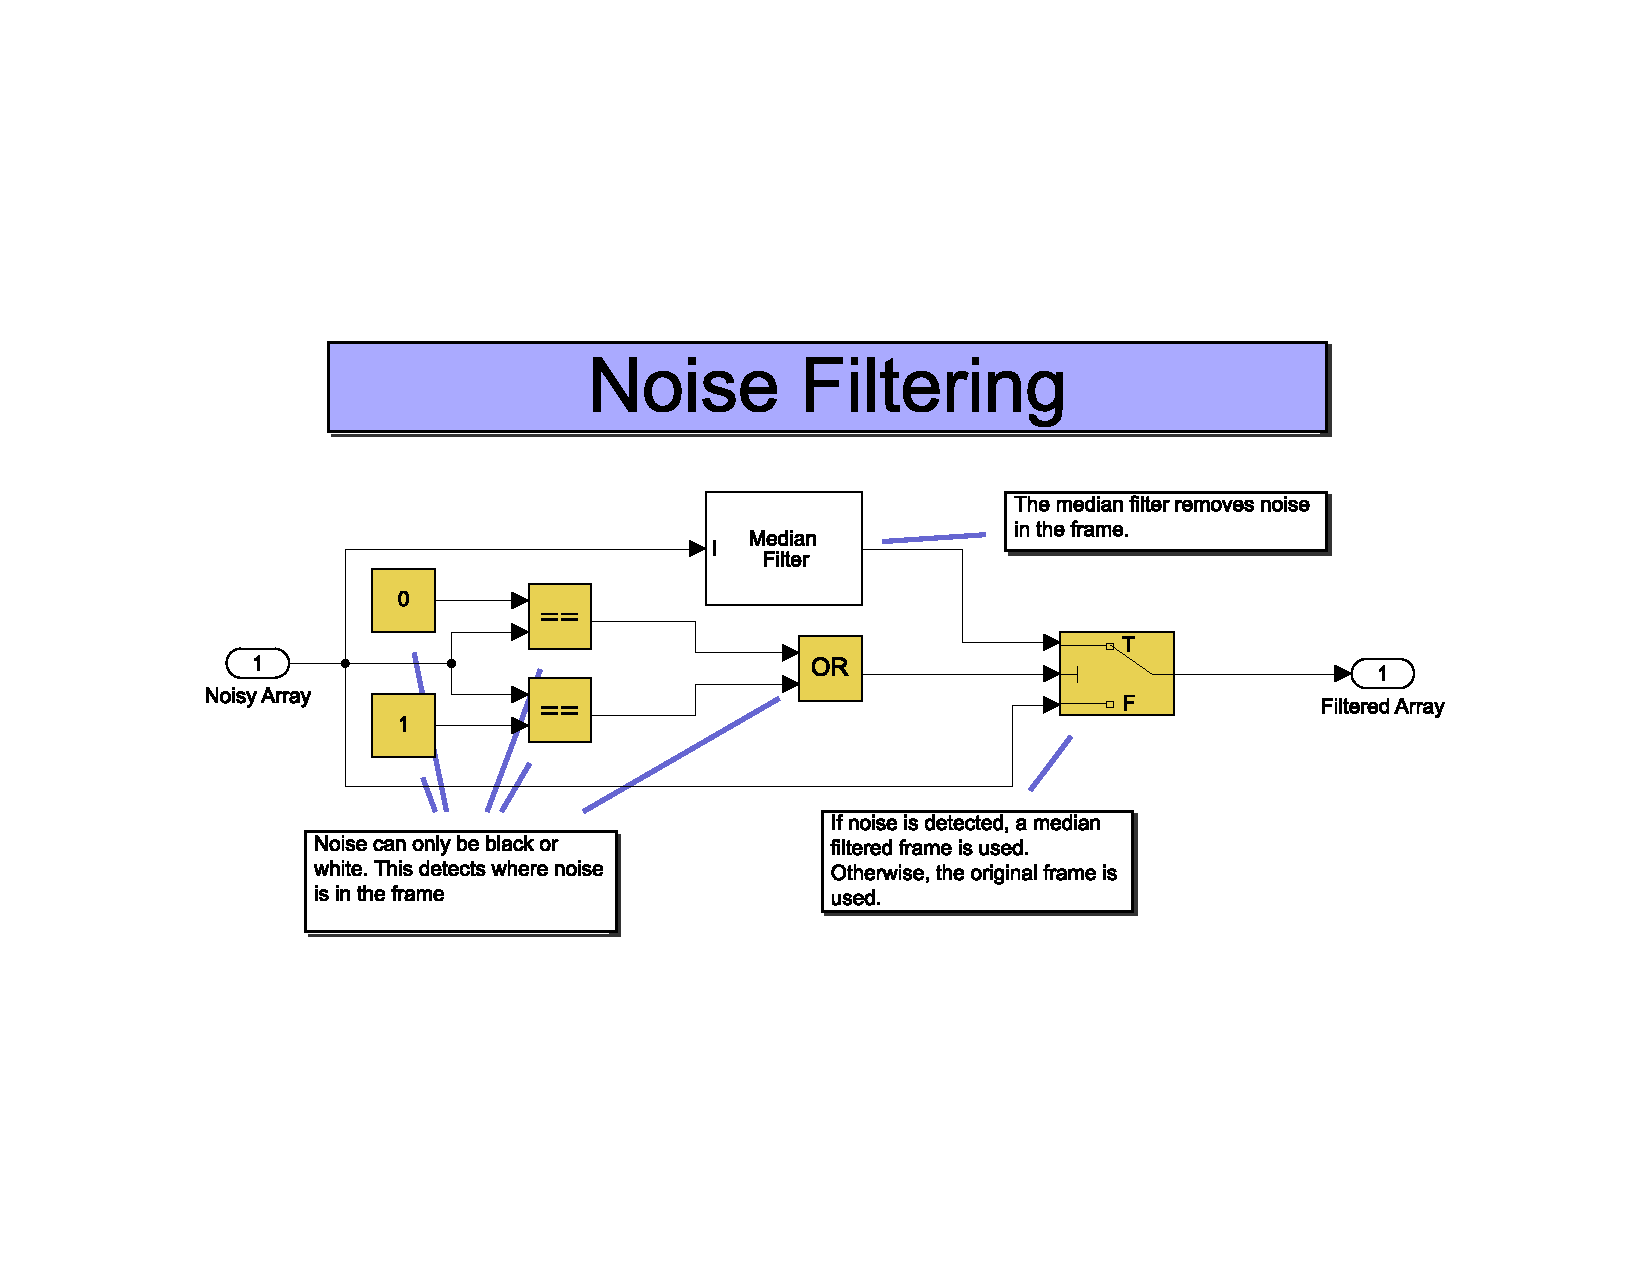
\includegraphics[width=\linewidth]{impl_dsgn_Noise Filtering}
    \caption{Noise Filtering using a modified median filter}
    \label{fig:medianFilter}
\end{figure}
 \par Each pixel of the input frame is checked to see if it is pure black or white to determine if noise is present in that location. To reduce noise in the image, a median filter\footnote{For reference on median filters, please reference\hyperlink{https://homepages.inf.ed.ac.uk/rbf/HIPR2/median.htm}{Spatial Filters - Median Filters by Robert Fisher, Simon Perkins, Ashley Walker, Erik Wolfart}} is used with neighborhood size of 3x3. Fig. \ref{fig:medianFilter} outlines the construction of this noise reduction system. Since this is a somewhat idealized proof of concept design, the pixel must meet the pure white or pure black criteria. In a more real life scenario, some margin should be factored to compensate for noise in transmission to the processing unit.
 \par If the pixel is not deemed to be noise, then the original pixel is passed through. However, if the pixel is deemed to be noisy,  then the median filtered pixel is passed through.
 \par This module is verified using the peak signal-to-noise-ratio compared to the reference image. This is done in the \verb!Verification! block. The PSNR is calculated using the mean-square-error or MSE. The MSE represents the amount the reference image differs from the test image, and PSNR is a measure of the peak error and is calculated by dividing the maximum data type range by the MSE. This document uses floating point, therefore the maximum range is one\cite{mathworks}.
 \subsubsection{Noise Identification Sub module}
 Noise identification is accomplished by averaging eight frames and isolating the parts of the frame that is the most common amongst the eight frames.
 \begin{figure}[H]
    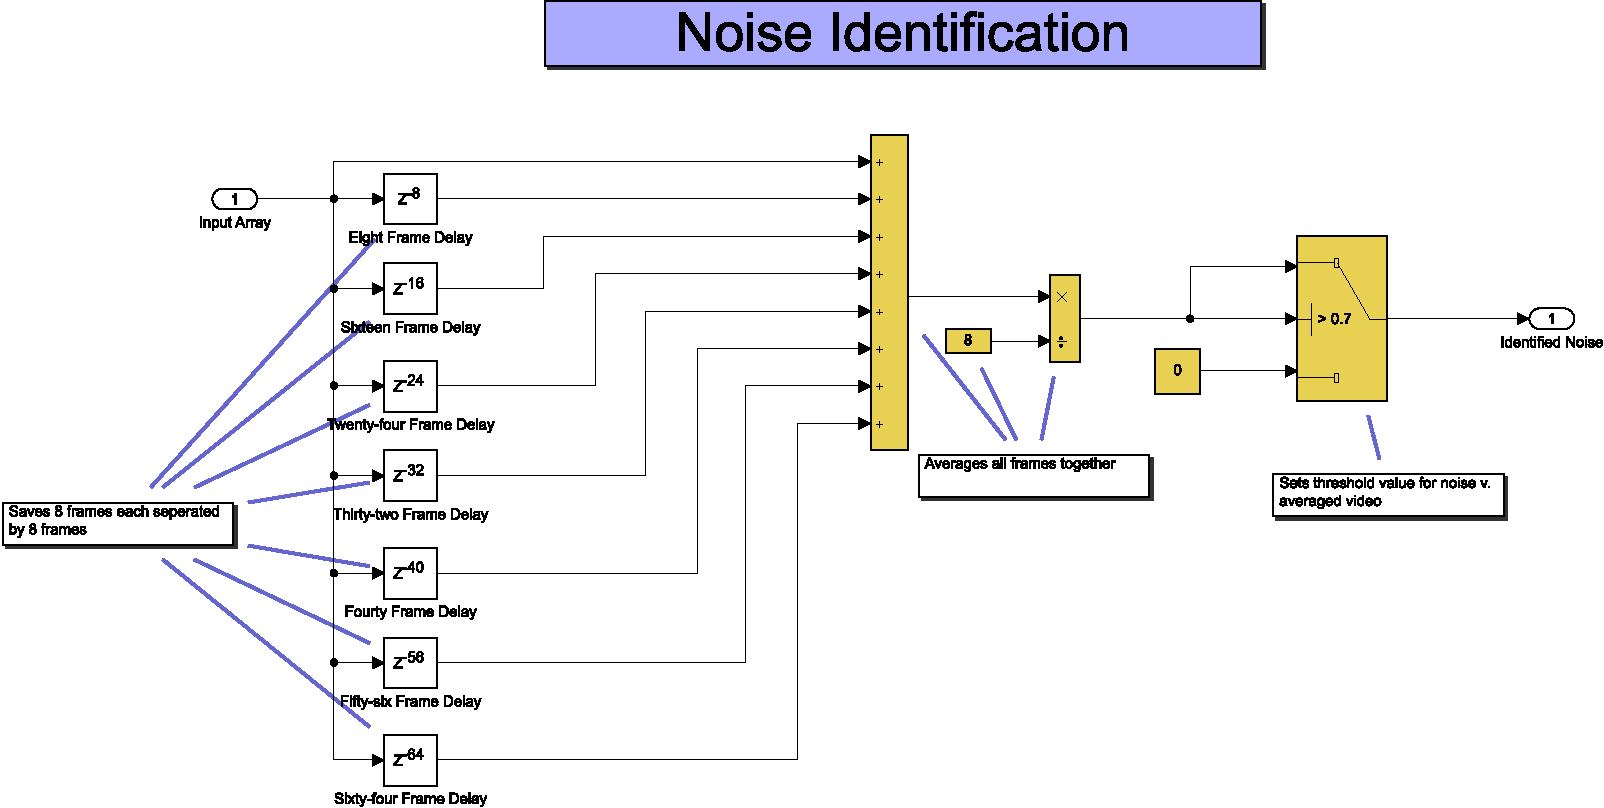
\includegraphics[width=\linewidth]{impl_dsgn_Noise Identification}
    \caption{Noise Identification}
    \label{fig:noiseID}
\end{figure}
